%!TEX root = ../tesi.tex

\chapter{Design Pattern}
\label{a:designpatterns}
Nel campo dell'Ingegneria del Software con Design Pattern si intende uno schema di progettazione del software utilizzato per risolvere un problema ricorrente.
Molti di questi schemi sono stai pensati per il paradigma di programmazione ad oggetti e descrivono, utilizzando ereditariet\`a e interfacce, le interazioni e relazioni tra oggetti e classi.

In questa appendice vengono esposte alcune note generali sui design pattern citati nel testo, sia che siano stati implementati direttamente o semplicemente coinvolti nello sviluppo del progetto di tesi perch\'e sfruttati dalle parti interessate del framework.
Nella trattazione viene descritto l'obbiettivo di ogni schema, l'utilit\`a, note implementative con schema \ac{UML} annesso e alcuni benefici della sua applicazione, vengono inoltre raggruppati per categoria cos{\`\i} come vengono presentati in \cite{book:designpattern}.

\section{Pattern Creazionali}
I pattern creazionali sono usati per creare un'astrazione sul processo di instanziazione degli oggetti, in modo da rendere il sistema indipendente da come gli oggetti vengono effettivamente creati. Questo tipo di pattern diviene importante quando un sistema dipende principalmente da oggetti composti da aggregati di componenti pi\`u piccole, rispetto ad oggetti gerarchici organizzati in base all'ereditariet\`a.

\subsection{Abstract Factory}
\label{sub:abstractfactory}
L'obbiettivo di questo pattern \`e fornire un'interfaccia per la creazione di famiglie di oggetti imparentati o dipendenti tra loro, eliminado la necessit\`a di specificare i nomi delle classi concrete all'interno del codice.

In questo modo un sistema pu\`o essere indipendente da come vengono creati gli oggetti concreti e pu\`o essere configurato per utilizzare diverse famiglie di oggetti a seconda delle necessit\`a. Un caso esemplificativo \`e quello di un tool per l'implementazione di interfacce grafiche che supporta diversi look-and-feel. L'utilizzo di un diverso look-and-feel comporta la definizione di una nuova famiglia di componenti grafiche le cui caratteristiche base sono per\`o fondamentalmente identiche: un pulsante pu\`o essere premuto e disegnato a schermo. L'applicazione dovrebbe essere appunto indipendente da come il pulsante viene istanziato, ma essere in grado di riconoscerlo per le sue funzionalit\`a.

\begin{figure}
\begin{center}
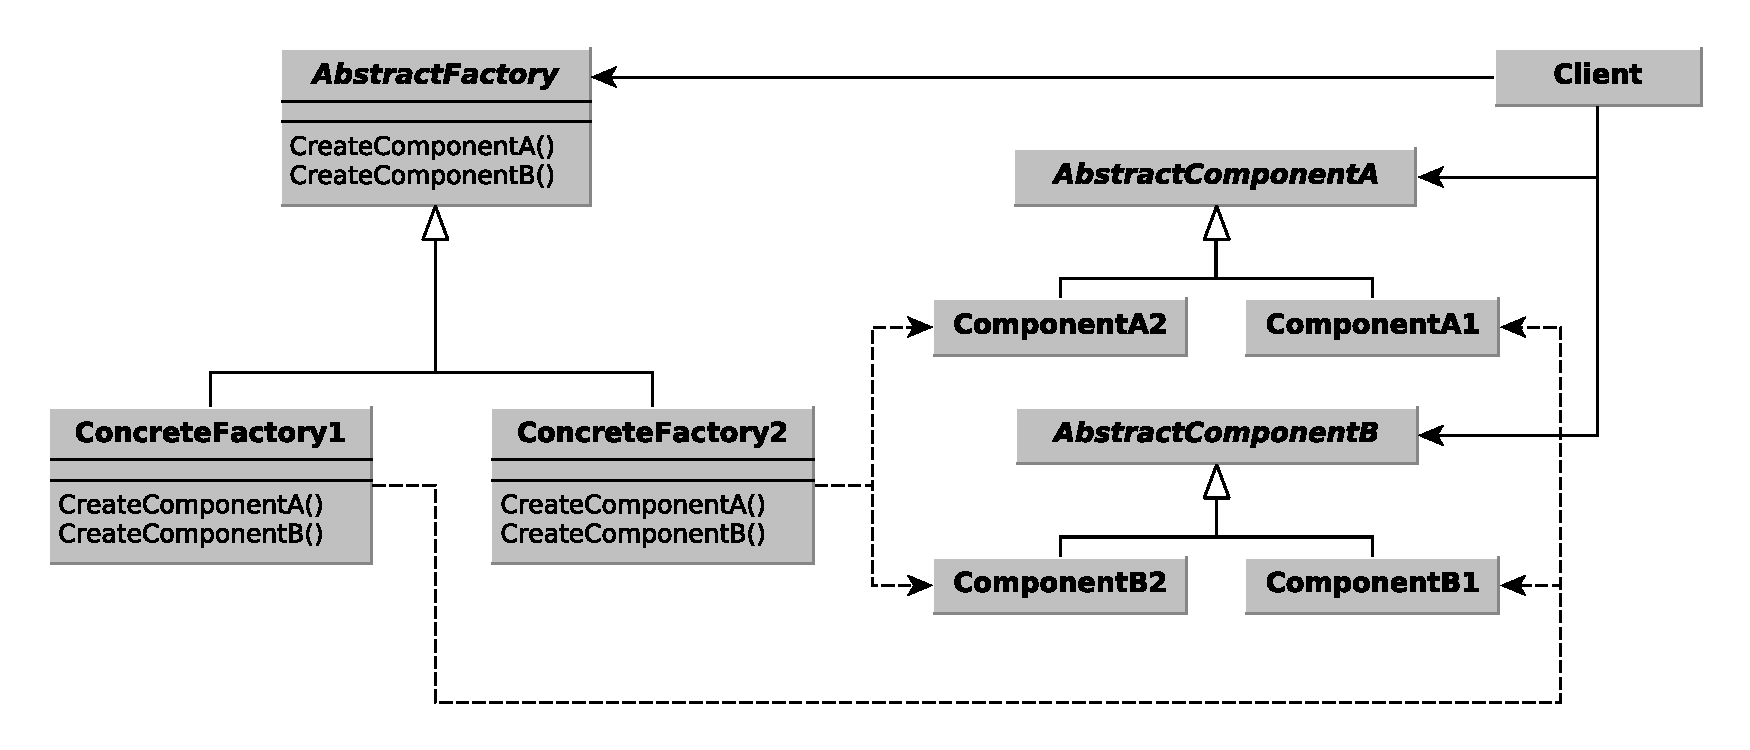
\includegraphics[width=13cm]{Immagini/AbstractFactoryPattern}
\caption{Struttura UML del pattern Abstract Factory.\label{f:abstractfactorypattern}} 
\end{center} 
\end{figure}

Per ottenere ci\`o \`e possibile definire una classe astratta o un'interfaccia differente per ogni componente generico desiderato, come \texttt{AbstractComponentA} e \texttt{AbstractComponentB} nella figura \ref{f:abstractfactorypattern}.
Si definisce poi una classe \texttt{AbstractFactory} astratta la cui funzione sia quella di creare istanze delle componenti astratte generiche. Se per ogni famiglia che si desidera implementare si generano sottoclassi concrete per ogni componente astratta e si definisce una Factory concreta in grado di istanziarle, come \texttt{ComponentA1} e \texttt{ConcreteFactory1} nell'esempio raffigurato, l'applicazione potr\`a utilizzare la Factory concreta che preferisce in modo del tutto indipendente da quale famiglia essa gestisce.

Questo schema permette di cambiare le famiglie di componenti in modo semplice e consente di isolare le classi concrete, dato che le componenti vengono utilizzate attraverso la loro interfaccia.

\subsection{Singleton}
\label{sub:singleton}
Lo scopo di questo pattern \`e garantire che di una determinata classe possa essere creata una unica istanza, fornendone un singolo punto di accesso globale.

L'utilit\`a di questo pattern \`e dovuta al fatto che spesso, all'interno di un'applicazione, ci sono servizi e funzionalit\`a condivise a cui deve essere associata una istanza univoca. Esempi classici in proposito sono il gestore del File System o il gestore dei servizi di stampa.

\begin{figure}
\begin{center}
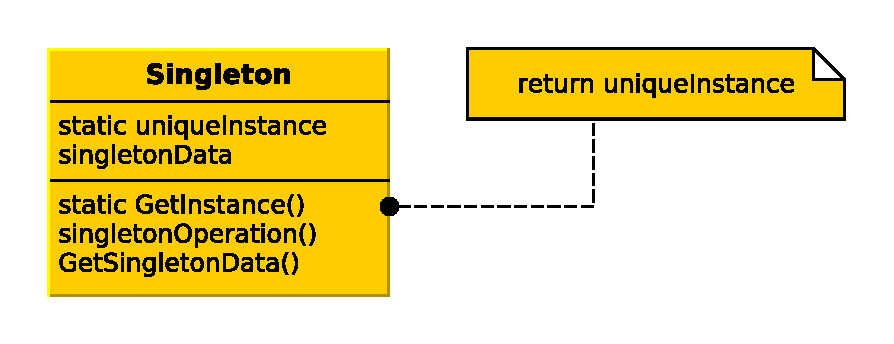
\includegraphics[width=12cm]{Immagini/SingletonPattern}
\caption{Struttura UML del pattern Singleton.\label{f:singletonpattern}}
\end{center} 
\end{figure}

Per ottenere questa propriet\`a spesso si delega alla classe stessa la responsabilit\`a di controllare la creazione delle propria istanza rendendo privato il suo costruttore, impedendo di fatto l'istanziazione dall'esterno. In figura \ref{f:singletonpattern} possiamo vedere lo schema \ac{UML} di una classe che utilizza il pattern in cui la classe possiede una unica istanza statica \texttt{uniqueIstance} accessibile solamente attraverso il metodo statico \texttt{GetInstance()}. 

Utilizzare questo schema consente di avere un pi\`u stretto controllo degli accessi alla risorsa, inoltre estendendo la classe \`e possibile raffinare le funzionalit\`a della risorsa e configurare l'applicazione a runtime per utilizzare l'istanza che serve per un caso specifico.

\section{Pattern Strutturali}
Questo tipo di pattern si occupa di come classi e oggetti vengono composte e interagiscono nella formazione di strutture pi\`u complesse. 
Un obbiettivo di questi pattern \`e permettere la composizione di oggetti complessi che uniscano le funzionalit\`a di moduli pi\`u piccoli rendendo quest'ultimi il pi\`u possibile riutilizzabili.

\subsection{Bridge}
\label{sub:bridge}
Questo pattern ha l'intento di disaccoppiare un'astrazione dalla sua implementazione in modo che entrambe possano evolversi in maniera indipendente.

Ci\`o \`e particolarmente utile quando si desidera evitare un legame permanente tra astrazione e implementazione, e si vuole permettere di scegliere o cambiare quest'ultima durante l'esecuzione. \'E utile inoltre quando sia astrazione che implementazione hanno la necessit\`a di essere estendibili attraverso sottoclassi. 

Un utile esempio per illustrare questo pattern \`e prendere in esame un ipotetico toolkit per interfacce grafiche, per renderlo il pi\`u possibile portabile su piattaforme diverse esso deve utilizzare un'astrazione che descriva le finestre in modo pi\`u generico possibile. Se per ottenere queste propriet\`a usassimo semplicemente una classe astratta \texttt{Window} da cui, usando l'ereditariet\`a, costruire sottoclassi specifiche per ogni sistema da supportare, otterremmo due svantaggi:
\begin{enumerate}
	\item Nell'evenienza di voler estendere la classe \texttt{Window} per coprire l'astrazione di altri tipi di finestra grafica esistente, per poter supportare tutte le piattaforme per cui esisteva una implementazione di \texttt{Window} dovremmo creare una sottoclasse specifica per ognuna di esse.
	\item Il codice del client diventa dipendente dalla piattaforma. Quando vi \`e la necessit\`a di creare una finestra, deve essere istanziata una classe concreta specifica e questo lega fortemente l'astrazione con l'implementazione utilizzata rendendo pi\`u complesso portare il codice del client su altre piattaforme.
\end{enumerate}
Per eludere questi problemi il pattern Bridge separa la gerarchia delle classi che appartengono all'astrazione da quella delle classi di implementazione. In cima alle due gerarchie vi sono le classi \texttt{Window} e \texttt{WindowImplementation}, che compongono il Bridge vero e proprio. La prima rappresenta l'astrazione della finestra che verr\`a utilizzata dal client, la seconda \`e invece l'interfaccia che un'implementazione concreta deve utilizzare per essere utilizzata dall'astrazione.
Come si pu\`o vedere nella figura \ref{f:bridgepattern}, la classe \texttt{Window} rimappa i propri metodi su quelli dell'interfaccia \texttt{WindowImplementation}, o con una combinazione di essi. Questi vengono chiamati su di una implementazione concreta di \texttt{WindowImplementation} di cui \texttt{Window} possiede un riferimento \texttt{imp}.

\begin{figure}
\begin{center}
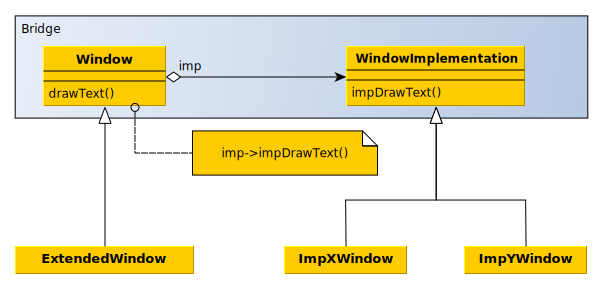
\includegraphics[width=12cm]{Immagini/BridgePattern}
\caption{Esempio di schema gerarchico dovuto all'applicazione del pattern Bridge.\label{f:bridgepattern}} 
\end{center} 
\end{figure}

L'utilizzo di questo schema permette di nascondere i dettagli implementativi ai client e di non avere effetti diretti su di esse quando l'implementazione cambia cos{\`\i} che il codice dei client non non ha un'effettiva necessit\`a di essere ricompilato. 

\subsection{Composite}
\label{sub:composite}
Lo scopo di questo pattern \`e consentire una gestione uniforme tra oggetti semplici ed oggetti compositi. Questo si traduce in una organizzazione degli oggetti in una struttura ad albero in cui ogni nodo \`e un oggetto aggregato e ogni foglia \`e un oggetto semplice.
Il nodo composito avr\`a al suo interno riferimenti ad oggetti figli che a loro volta possono essere semplici o compositi.

Spesso si desidera poter trattare oggetti composti nello stesso modo in cui gestiamo le sue componenti ignorando come siano effettivamente implementate le loro funzionalit\`a, un esempio significativo sono le interfacce grafiche in cui \`e comodo poter gestire gruppi di componenti, come pulsanti o etichette, in modo unitario come se si trattasse di una componente singola.

\begin{figure}
\begin{center}
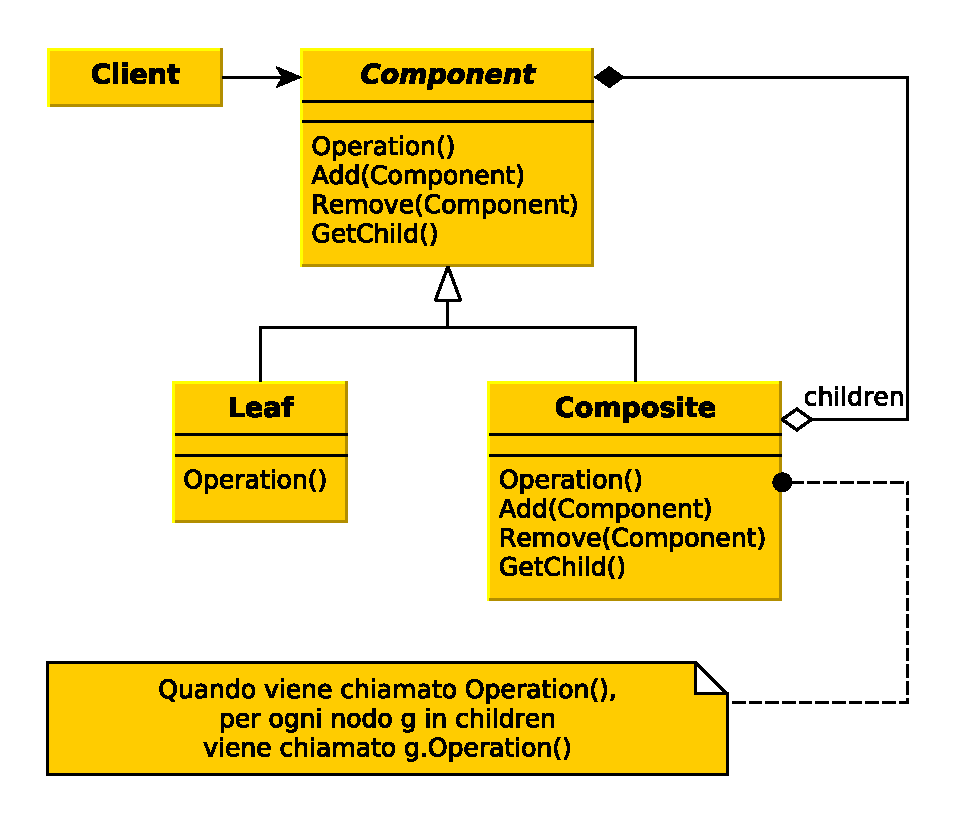
\includegraphics[width=10cm]{Immagini/CompositePattern}
\caption{Struttura UML del pattern Composite.\label{f:compositepattern}} 
\end{center} 
\end{figure}

Una metodologia per ottenere questo tipo di interazione \`e l'utilizzo di una classe astratta che rappresenti sia gli oggetti semplici, o primitive, sia gli oggetti composti, o contenitori. Nello schema \ac{UML} in figura \ref{f:compositepattern}, la classe astratta \texttt{Component} rappresenta sia oggetti foglia \texttt{Leaf} che nodi \texttt{Composite}. Un client pu\`o richiamare indifferentemente i metodi di interfaccia di un oggetto sottoclasse di \texttt{Component} sia che si tratti di un una foglia o di un nodo. Nel caso di una foglia il metodo risponder\`a direttamente in maniera appropriata mentre nel caso di un nodo verr\`a richiamato lo stesso metodo per tutti gli oggetti figli.

L'utilizzo di questo pattern consente di rendere meno complessi i moduli che utilizzano le strutture composite, che non hanno bisogno di sapere se stiano trattando una foglia o un nodo dell'albero. Consente inoltre di aggiungere in modo semplice nuovi componenti senza laboriosi interventi sul codice pre-esistente.
% TODO: valutare una citazione sul principio OpenClose SOLID


\section{Pattern Comportamentali}
I pattern comportamentali riguardano gli algoritmi e la suddivisione delle responsabilit\`a tra gli oggetti, per fare ci\`o non si limitano solamente a descrivere i rapporti tra oggetti e classi, ma anche attraverso schemi di comunicazione tra di essi. Questi schemi permettono di descrivere complessi flussi di controllo spostando l'attenzione da essi alle connessioni fra gli oggetti.

\subsection{State}
\label{sub:state}
Il pattern State ha come scopo quello di consentire ad un oggetto di cambiare il proprio comportamento durante l'esecuzione, in base alle variazioni del proprio stato interno.

Esempi di questo tipo di necessit\`a possono essere trovati in oggetti che gestiscono connessioni e che devono rispondere in modo diverso in base allo stato della connessione stessa, oppure nella costruzione di macchine a stati che implementano algoritmi di controllo.

\begin{figure}
\begin{center}
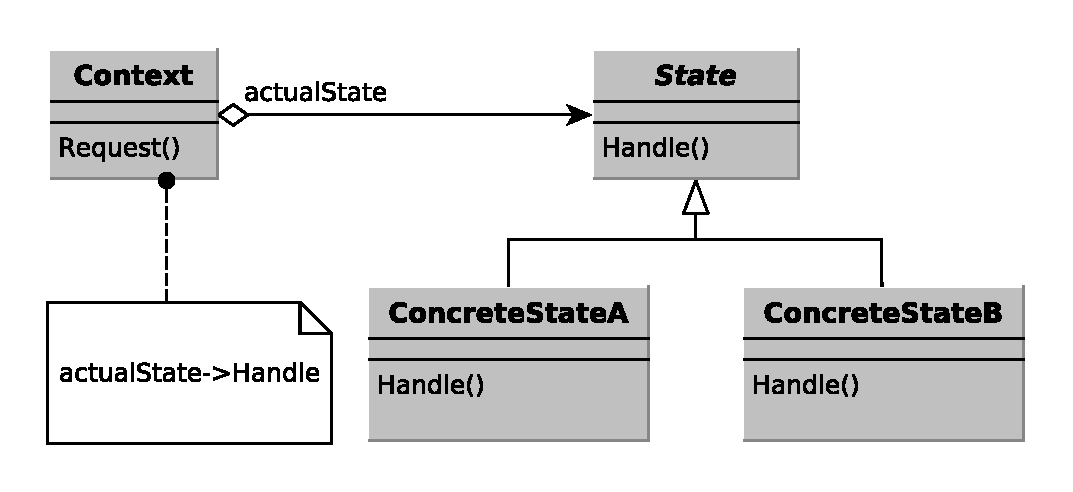
\includegraphics[width=12cm]{Immagini/StatePattern}
\caption{Schema UML del pattern State.\label{f:statepattern}} 
\end{center} 
\end{figure}

La figura \ref{f:statepattern} mostra in uno schema \ac{UML} la struttura del pattern. La classe \texttt{Context} rappresenta l'interfaccia che l'oggetto a stato variabile presenta verso i client. Al suo interno mantiene una istanza (\texttt{actualState}) di una sottoclasse concreta della classe \texttt{State}.
La classe astratta \texttt{State} definisce un'interfaccia per incapsulare il comportamento associato ad uno stato.
Le sottoclassi concrete di \texttt{State} sono associate ad un effettivo stato e implementano il comportamento che l'oggetto \texttt{Context} assume in quel caso.
Quando i client effettuano richieste all'oggetto \texttt{Context} attraverso la sua interfaccia, viene richiamato il metodo di interfaccia dell'istanza concreta \texttt{actualState}.
Il pattern non definisce dove vada inserita la logica di cambiamento di stato, ma in generale \`e pi\`u flessibile consentire alle sottoclassi di \texttt{State} la definizione dello stato successivo.

L'applicazione del pattern consente di eliminare lunghe e complesse parti di codice in cui una sequenza di istruzioni condizionali determinano le istruzioni da eseguire in base allo stato dell'oggetto. Consente inoltre di isolare il codice specifico relativo ad uno stato in un singolo oggetto permettendo l'aggiunta di nuovi stati e transizioni semplicemente definendo nuove classi.